\chapter{Linear Algebra \cite{mfml-1}}

\section{Groups ( $G = (\mathbb{G}, \otimes)$ ) \cite{mfml-1}}\label{lin-alg-Groups}

Consider a set $\mathbb{G}$ and an operation $\otimes$ : $\mathbb{G} \times \mathbb{G} \to \mathbb{G}$ group defined on $\mathbb{G}$. Then $G := (\mathbb{G}, \otimes)$ is called a group if the following hold:

\begin{table}[H]
    \begin{tabular}{l p{10cm}}
        Closure of $\mathbb{G}$ under $\otimes$ & $\forall x,y \in \mathbb{G} : x \otimes y \in \mathbb{G}$ \\
        Associativity & $\forall x,y,z \in \mathbb{G}:(x \otimes y) \otimes z = x \otimes (y \otimes z) $ \\
        Neutral Element & $\exists e \in \mathbb{G} \text{ , } \forall x\in \mathbb{G}: x \otimes e = e \otimes x = x$ \\
        Inverse Element & $\forall x\in \mathbb{G} \text{ , } \exists y \in \mathbb{G}: x\otimes y = y\otimes x = e$ where $e$ is the neutral element. ( $y = x^{-1}$ and $x = y^{-1}$ ) \\
    \end{tabular}
\end{table}

\begin{enumerate}
    \item Inverse of element is w.r.t. operation $\otimes$, does not necessarily mean $\displaystyle\dfrac{1}{x}$.
\end{enumerate}

Examples:
\begin{enumerate}
    \item $(\mathbb{N}_0, +)$ is \textbf{NOT} a group: Although $(\mathbb{N}_0, +)$ possesses a neutral element ($0$), the inverse elements are missing. ($\mathbb{N}_0 = \mathbb{N} \cup {0} $)

    \item $(\mathbb{Z}, \cdot)$ is \textbf{NOT} a group: Although $(\mathbb{Z}, \cdot)$ contains a neutral element ($1$), the inverse elements for any $z \in \mathbb{Z}$, $z \neq \pm 1$, are missing.

    \item $(\mathbb{R}, \cdot)$ is \textbf{NOT} a group since $0$ does not possess an inverse element.

    
\end{enumerate}









\section{Abelian Group \cite{mfml-1}}\label{Abelian Group}

All properties of Group (SEE: \fullref{lin-alg-Groups}) with additional condition/ property:

\begin{table}[H]
    \begin{tabular}{l l}
        commutative \hspace{0.5cm} & $\forall x,y \in \mathbb{G}:x\otimes y = y\otimes x$ \\
    \end{tabular}
\end{table}

Examples:
\begin{enumerate}
    \item $(\mathbb{Z}, +)$ is an Abelian group.
    \item $(\mathbb{R}\textbackslash {0}, ·)$ is Abelian.
    \item $(\mathbb{R}^n, +)$, $(Z^n, +)$, $n \in N$ are Abelian if $+$ is defined componentwise, i.e., 
    \[
        (x_1, \cdots , x_n) + (y_1, \cdots , y_n) = (x_1 + y_1, \cdots , x_n + y_n)
    \]
    Then, $(x_1, \cdots , x_n)^{-1} := (-x_1, \cdots , -x_n)$ is the inverse element and $e = (0, \cdots , 0)$ is the neutral element.
    \item $(\mathbb{R}^{m\times n}, +)$, the set of $m \times n$-matrices is Abelian (with componentwise addition)
\end{enumerate}










\section{General Linear Group ( $GL(n,\mathbb{R})$ ) \cite{mfml-1}}\label{General Linear Group}

The set of regular (invertible) matrices $A \in \mathbb{R}^{n \times n}$ is a group with respect to matrix multiplication as defined in and is called \textbf{general linear group} $GL(n, \mathbb{R})$.\\
However, general linear group since matrix multiplication is not commutative, the group is \textbf{NOT} Abelian.

\begin{table}[h]
    \begin{tabular}{l p{7cm}}
        Closure & follow directly from the definition of matrix multiplication \\
        
        associativity & follow directly from the definition of matrix multiplication \\

        Neutral element & The identity matrix $\mathbb{I}_n$ is the neutral element with respect to matrix multiplication "$\cdot$" in $(\mathbb{R}^{n\times n}, \cdot)$ \\

        Inverse element & If the inverse exists ($\mathbf{A}$ is regular), then $\mathbf{A}^{-1}$ is the inverse element of $\mathbf{A} \in \mathbb{R}^{n\times n}$, and in exactly this case $(\mathbb{R}^{n\times n}, \cdot)$ is a group, called the \textbf{general linear group}\\
        
    \end{tabular}
\end{table}














\section{Vector Spaces ( $V = (\mathbb{V}, +, \cdot)$ ) \cite{mfml-1}}\label{Vector Spaces}

A real-valued vector space $V = (\mathbb{V}, +, \cdot)$ is a set $\mathbb{V}$ with two operations:

\begin{table}[H]
    \centering
    \begin{tabular}{l l}
        $+$ & $: \mathbb{V} \times \mathbb{V} \to \mathbb{V}$ \\

        $\cdot$ & $: \mathbb{R} \times \mathbb{V} \to \mathbb{V}$ \\

    \end{tabular}
\end{table}

where,
\begin{enumerate}
    \item $(\mathbb{V}, +)$ is an Abelian group (SEE: \fullref{Abelian Group})
    \item Distributivity:
    \begin{enumerate}
        \item $\forall \lambda \in \mathbb{R}, \mathbf{x,y}\in \mathbb{V} : \lambda\cdot(\mathbf{x+y}) = \lambda\cdot\mathbf{x} + \lambda\cdot\mathbf{y}$
        
        \item $\forall \lambda,\psi \in \mathbb{R}, \textbf{x}\in \mathbb{V} : (\lambda + \psi) \cdot\textbf{x} = \lambda\cdot\textbf{x} + \psi\cdot\textbf{x}$
        
    \end{enumerate}

    \item Associativity (outer operation): $\forall \lambda,\psi\in\mathbb{R}, \mathbf{x}\in\mathbb{V}: \lambda\cdot(\psi\cdot\mathbf{x}) = (\lambda\psi)\cdot\mathbf{x}$

    \item Neutral element with respect to the outer operation: $\forall \mathbf{x}\in\mathbb{V}:1\cdot\mathbf{x}=\mathbf{x}$
\end{enumerate}
\vspace{0.3cm}

\textbf{Notes:}
\begin{enumerate}
    \item The elements $\mathbf{x}\in\mathbb{V}$ are called \textbf{vectors}\indexlabel{vectors}.
        \item The vector spaces $\mathbb{R}^n$, 
        \begin{enumerate}
            \item $\mathbb{R}^{n\times 1}$, $\mathbb{R}^{1\times n}$ are only different in the way we write vectors
        
            \item default: n-tuples as \textbf{column vectors}\indexlabel{column vectors} ($\mathbb{R}^n = \mathbb{R}^{n \times 1}$) : $\mathbf{x}$
    
            \item default: n-tuples as \textbf{row vectors}\indexlabel{row vectors} ($\mathbb{R}^{1 \times n}$) : $\mathbf{x}^\top$
        \end{enumerate}

    \item The \textbf{neutral element} of $(\mathbb{V}, +)$ is the zero vector $0 = [0, \cdots, 0]^T$ \\
    the inner operation $+$ is called \textbf{vector addition}\indexlabel{vector addition}.

    \item The elements $\lambda\in\mathbb{R}$ are called \textbf{scalars}\indexlabel{scalars} and the outer operation $\cdot$ is a \textbf{multiplication by scalars}.

    \item “vector multiplication” $\mathbf{ab, a, b} \in \mathbb{R}^n$, is \textbf{NOT} defined

    \item we could define an \textbf{element-wise multiplication}, such that $\mathbf{c = ab}$ with $c_j = a_j \times b_j$

    \item $\mathbb{V} = \mathbb{R}^n, n \in \mathbb{N}$ is a vector space with operations defined as follows:
    \begin{enumerate}
        \item \textbf{Addition}:\\ $\mathbf{x+y} = (x_1, \cdots, x_n)+(y_1, \cdots, y_n) = (x_1+y_1, \cdots, x_n+y_n) \forall \mathbf{x, y} \in \mathbb{R}^n$

        \item \textbf{Multiplication by scalars}:\\ $\lambda\mathbf{x} = \lambda(x_1, \cdots, x_n) = (\lambda x_1, \cdots, \lambda x_n) \forall \lambda \in \mathbb{R}, \mathbf{x} \in \mathbb{R}^n$
        
    \end{enumerate}

    \item $\mathbb{V} = \mathbb{R}^{m\times n}, m, n \in \mathbb{N}$ is a vector space with:
    \begin{enumerate}
        \item \textbf{Addition} is defined element-wise $\forall \mathbf{A, B} \in \mathbb{V}$: 
        \[
            \mathbf{A + B} = \begin{bmatrix}
                a_{11} + b_{11} & \cdots & a_{1n} + b_{1n} \\
                \vdots & & \vdots \\
                a_{m1} + b_{m1} & \cdots & a_{mn} + b_{mn} \\
            \end{bmatrix}
        \]

        \item \textbf{Multiplication by scalars} $\forall \lambda\in\mathbb{R}, \mathbf{A}\in\mathbb{R}^{m\times n}$:
        \[
            \lambda\mathbf{A} = \begin{bmatrix}
                \lambda a_{11} & \cdots & \lambda a_{1n} \\
                \vdots & & \vdots \\
                \lambda a_{m1} & \cdots & \lambda a_{mn} \\
            \end{bmatrix}
        \]
    \end{enumerate}


\end{enumerate}













\section{Vector Subspaces/ linear subspace ( $U = (\mathbb{U}, +, \cdot)$ ) \cite{mfml-1}}\label{Vector Subspaces/ linear subspace}
Let $V = (\mathbb{V}, +, \cdot)$ be a vector space and $\mathbb{U} \subseteq \mathbb{V}$, $\mathbb{U} \neq \varnothing$. Then $U = (\mathbb{U}, +, \cdot)$ is called vector subspace of $V$ (or linear subspace) if $U$ is a vector space with the vector space operations $+$ linear subspace and $\cdot$ restricted to $\mathbb{U} \times \mathbb{U}$ and $\mathbb{R} \times \mathbb{U}$. We write $U \subseteq V$ to denote a subspace $U$ of $V$.

\begin{enumerate}
    \item Vector subspace inherits Abelian group properties, the distributivity, the associativity and the neutral element from the vector space.

    \item To determine whether $U = (\mathbb{U}, +, \cdot)$ is a subspace of $V$ we still do need to show:
    \begin{enumerate}
        \item $\mathbb{U} \neq \varnothing$, in particular: $\mathbf{0} \in \mathbb{U}$ (zero vector)
        \item Closure of $U$:
        \begin{enumerate}
            \item With respect to the \textbf{outer operation}: $\forall\lambda \in \mathbb{R}, \forall\mathbf{x} \in \mathbb{U} : \lambda \mathbf{x} \in \mathbb{U}$
            \item With respect to the \textbf{inner operation}: $\forall\mathbf{x, y} \in \mathbb{U} : \mathbf{x + y} \in \mathbb{U}$
        \end{enumerate}
    \end{enumerate}

    \item For every vector space $V$, the trivial subspaces are $V$ itself and ${\mathbf{0}}$.
    
\end{enumerate}








\section{Dimension of Vector Space ( $\dim(V)$ ) \cite{mfml-1}}\label{lin-alg: Dimension-vector-space}

\begin{enumerate}
    \item The dimension of $V$ is the number of basis vectors of $V$, and we write $\dim(V)$.

    \item If $U \subseteq V$ is a subspace of $V$, then $\dim(U) \leq \dim(V)$ and $\dim(U) = \dim(V)$ if and only if $U = V$.

    \item the dimension of a vector space can be thought of as the number of independent directions in this vector space.

    \item The dimension of a vector space is \textbf{NOT} necessarily the number of elements in a vector.\\
    \textbf{Example}: $V = \rcmdXspan[\begin{bmatrix}0\\1\end{bmatrix}]$ is one-dimensional, although the basis vector possesses two elements.
    
\end{enumerate}









\section{Linear Combination \cite{mfml-1}}\label{Linear Combination}
Consider a vector space $V$ and a finite number of vectors $\mathbf{x_1, \cdots , x_k} \in V$ . Then, every $\mathbf{v} \in V$ of the form
\[
    \hfill
    \displaystyle
    \mathbf{v} = \lambda_1 \mathbf{x}_1 + \cdots + \lambda_k \mathbf{x}_k = \sum_{i=1}^{k} \lambda_i \mathbf{x}_i \in V
    \hfill
\] 
with $\lambda_1, \cdots, \lambda_k \in \mathbb{R}$ is a linear combination of the vectors $\mathbf{x_1, \cdots, x_k}$.

\begin{enumerate}
    \item The $\mathbf{0}$-vector can always be written as the linear combination of $k$ vectors $\mathbf{x_1, \cdots, x_k}$ because $\displaystyle\mathbf{0} = \sum_{i=0}^{k} 0\cdot\mathbf{x_i}$ is always true.
\end{enumerate}






\section{Linear (In)dependence \cite{mfml-1}}\label{Linear (In)dependence}

Let us consider a vector space $V$ with $k \in \mathbb{N}$ and $\mathbf{x_1, \cdots, x_k} \in V$. If there is a non-trivial linear combination, such that $0 = \displaystyle\sum^k_{i=1} \lambda_i\mathbf{x_i}$ with at least one $\lambda_i \neq 0$, the vectors $\mathbf{x_1, \cdots, x_k}$ are \textbf{linearly dependent}. \\If only the trivial solution exists, i.e., $\lambda_1 = \cdots = \lambda_k = 0$ the vectors $\mathbf{x_1, \cdots, x_k}$ are \textbf{linearly independent}.

\vspace{0.3cm}
\noindent\textbf{Properties}:
\begin{enumerate}
    \item $k$ vectors are either linearly dependent or linearly independent. There is no third option.

    \item If at least one of the vectors $\mathbf{x_1, \cdots, x_k}$ is $\mathbf{0}$ then they are linearly dependent. The same holds if two vectors are \textbf{identical}.

    \item The vectors $\{\mathbf{x_1, \cdots, x_k} : \mathbf{x_i} \neq \mathbf{0}, i = 1, \cdots, k\}, k \geq 2$, are linearly dependent if and only if (at least) one of them is a linear combination of the others. In particular, if one vector is a multiple of another vector, i.e., $\mathbf{x_i} = \lambda\mathbf{x_j} , \lambda \in \mathbb{R}$ then the set $\{\mathbf{x_1, \cdots, x_k} : \mathbf{x_i} \neq \mathbf{0}, i = 1, \cdots, k\}$ is \textbf{linearly dependent}.

    \item A practical way of checking whether vectors $\mathbf{x_1, \cdots, x_k} \in V$ are linearly independent is to use Gaussian elimination: 
    \begin{enumerate}
        \item Write all vectors as columns of a matrix A and perform Gaussian elimination until the matrix is in row echelon form (the reduced row-echelon form is unnecessary here)
        
        \item The pivot columns indicate the vectors, which are linearly independent of the vectors on the left. Note that there is an ordering of vectors when the matrix is built.

        \item The non-pivot columns can be expressed as linear combinations of the pivot columns on their left.

        \item All column vectors are linearly independent if and only if all columns are pivot columns. If there is at least one non-pivot column, the columns (and, therefore, the corresponding vectors) are \textbf{linearly dependent}.
    \end{enumerate}

    \item Consider a vector space $V$ with $k$ linearly independent vectors $\mathbf{b_1, \cdots, b_k}$ and $m$ linear combinations
    \begin{enumerate}
        \item \( \displaystyle \mathbf{x}_1  = \sum_{i=1}^{k} \bm{\lambda}_{1i} \mathbf{b}_i  \quad\quad\cdots\quad\quad \mathbf{x}_m = \sum_{i=1}^{k} \bm{\lambda}_{im} \mathbf{b}_i \)

        \item $\mathbf{B} = [\mathbf{b_1, \cdots, b_k}]$ as the matrix whose columns are the linearly independent vectors $\mathbf{b_1, \cdots, b_k}$
        \[
            \mathbf{x}_j = \mathbf{B{\bm{\lambda}}}_j \quad\quad\quad\quad \bm{\lambda}_j = [\lambda_{1j}, \cdots, \lambda_{kj}]^\top
            \hfill (j=1, \cdots,m)
        \]

        \item \( \displaystyle \sum_{j=1}^{m} \psi_j \mathbf{x}_j = \sum_{j=1}^{m} \psi_j \mathbf{B}\bm{\lambda}_j = \mathbf{B}\sum_{j=1}^{m} \psi_j \bm{\lambda}_j \)\\
        This means that $\{\mathbf{x_1, \cdots, x_m}\}$ are linearly independent if and only if the column vectors $\{\bm{\lambda_1, \cdots, \lambda_m}\}$ are linearly independent.

    \end{enumerate}

    \item In a vector space $V$, $m$ linear combinations of $k$ vectors $\mathbf{x_1, \cdots, x_k}$ are linearly dependent if $m > k$.
\end{enumerate}







\section{Generating Set ( $\mathbb{A}$ ) \cite{mfml-1}}\label{Generating Set}
Consider a vector space $V = (\mathbb{V}, +, \cdot)$ and set of vectors $\mathbb{A} = \mathbf{\{x_1, \cdots , x_k\}} \subseteq \mathbb{V}$. If every vector $v \in V$ can be expressed as a linear combination of $\mathbf{x_1, \cdots , x_k}$, $\mathbb{A}$ is called a generating set of $V$.

\begin{enumerate}
    \item Generating sets are sets of vectors that span vector (sub)spaces, i.e., every vector can be represented as a linear combination of the vectors in the generating set.
\end{enumerate}













\section{Span ( $\rcmdXspan[\mathbb{A}]$ ) \cite{mfml-1}} \label{lin-alg: Span}
The set of all linear combinations of vectors in a generating set $\mathbb{A}$ is called the span of $\mathbb{A}$. If $\mathbb{A}$ spans the vector space $V$, we write 
\[
    \hfill
    V = \rcmdXspan[\mathbb{A}]
    \hfill
    \text{(or)}
    \hfill
    V = \rcmdXspan[\mathbf{x_1, \cdots , x_k}]
    \hfill
\]













\section{Basis ( $\mathbb{B}$ ) \cite{mfml-1}}\label{lin-alg: Basis}
Consider a vector space $V = (\mathbb{V}, +, \cdot)$ and $\mathbb{A} \subseteq \mathbb{V}$. A generating set $\mathbb{A}$ of $V$ is called \textbf{minimal} if there exists no smaller set $\tilde{\mathbb{A}} \not\subseteq \mathbb{A} \subseteq V$ that spans $V$. Every linearly independent generating set of $V$ is minimal and is called a basis of $V$.

\vspace{0.2cm}
Let $V = (\mathbb{V}, +, \cdot)$ be a vector space and $\mathbb{B} \subseteq \mathbb{V}, \mathbb{B} \neq \varnothing$. Then, the following statements are equivalent:

\begin{enumerate}
    \item $\mathbb{B}$ is a basis of $V$.
    
    \item $\mathbb{B}$ is a minimal generating set.
    
    \item $\mathbb{B}$ is a maximal linearly independent set of vectors in $V$, i.e., adding any other vector to this set will make it linearly dependent.

    \item Every vector $\mathbf{x} \in V$ is a linear combination of vectors from $\mathbb{B}$, and every linear combination is unique, i.e., with \( \displaystyle \mathbf{x} = \sum_{i=1}^{k} \lambda_i \mathbf{b}_i = \sum_{i=1}^{k} \psi_i \mathbf{b}_i \) and $\lambda_i, \psi_i \in \mathbb{R}, \mathbf{b}_i \in \mathbb{B}$, it follows that $\lambda_i = \psi_i$, $i=1,\cdots,k$

    
\end{enumerate}

\vspace{0.2cm}
\textbf{Note}:
\begin{enumerate}
    \item Every vector space $V$ possesses a basis $\mathbb{B}$. 
    
    \item There is \textbf{NO} unique basis. 
    
    \item All bases possess the same number of elements, the \textbf{basis vectors}\indexlabel{basis vectors}.

    \item A basis effectively defines a \textbf{coordinate system}. (SEE: \fullref{Coordinate vector})
\end{enumerate}

\subsection{Finding Basis \cite{mfml-1}}
A basis of a subspace $U = \rcmdXspan[\mathbf{x_1, \cdots, x_m}] \subseteq \mathbb{R}^n$ can be found by executing the following steps:
\begin{enumerate}
    \item Write the spanning vectors as columns of a matrix $\mathbf{A}$
    \item Determine the row-echelon form of $\mathbf{A}$
    \item The spanning vectors associated with the pivot columns are a basis of $U$
\end{enumerate}


\subsection{Ordered Basis ( $\mathit{B}$ ) \cite{mfml-1}}\label{ordered basis}
$n$-tuple an \textbf{ordered basis} of $\mathbf{V}$: $\mathit{B} = (\mathbf{b_1, \cdots, b_n})$


\subsection{Orthogonal Basis (OGB) \cite{mfml-1}}\label{Orthogonal Basis (OGB)}
Consider an $n$-dimensional vector space $V$ and a basis ${b_1, \cdots , b_n}$ of $V$. If $\langle b_i , b_j \rangle = 0 i \neq j$, then the basis is called the \textbf{orthogonal basis}.


\subsection{Orthonormal Basis (ONB) \cite{mfml-1}}\label{Orthonormal Basis (ONB)}
Orthogonal basis which satisfies $\langle b_i , b_i \rangle = 1$, then the basis is called the \textbf{orthonormal basis}.

To get ONB from OGB, normalize the individual vectors of OGB, and it will become ONB.

\subsection*{Getting ONB \cite{mfml-1}}
$\mathbf{B} = [\mathbf{b}_1, \cdots, \mathbf{b}_n]$\\
$\mathbf{b}_1, \cdots, \mathbf{b}_n$ : non-orthogonal and un-normalized basis vectors

\subsection{ONB using Gaussian Elimination Process \cite{jstor/2324877-Gram-Schmidt-Orthogonalization-by-Gauss-Elimination}}\label{ONB using Gaussian Elimination Process}

\begin{enumerate}
    \item Apply Gaussian Elimination to $[\mathbf{BB}^\top|\mathbf{B}]$ or $[\mathbf{B^\top B}|\mathbf{B}^\top]$

    \item Right side of the result will be set of mutually orthogonal vectors
\end{enumerate}

\subsection{Gram-Schmidt Process/ Gram-Schmidt Algorithm/ Gram-Schmidt Orthogonalization \cite{mfml-1}}\label{Gram-Schmidt Process/ Gram-Schmidt Algorithm/ Gram-Schmidt Orthogonalization}

Orthogonal Basis (OGB) : $(\mathbf{u}_1, \cdots ,\mathbf{u}_n)$

\subsubsection*{Method 1 \cite{mfml-1}}

\begin{align*}
    \mathbf{u}_1 &:= \mathbf{b}_1 \\
    \mathbf{u}_k &:= \mathbf{b}_k - \pi_{span[\mathbf{u_1, \cdots, u_{k-1}}]}(\mathbf{b}_k) \\
\end{align*}

SEE: projection - TODO

\subsubsection*{Method 2 \cite{youtube/UOZjINOGLog-Gram-Schmidt-Orthogonalisation-Process}}

\begin{align*}
    \displaystyle
    \mathbf{u}_1 &:= \dfrac{\mathbf{b}_1}{||\mathbf{b}_1||}\\
    \gamma_k &:= \mathbf{b}_k - \left( \sum_{i=1}^{k-1} \langle \mathbf{b}_k, \mathbf{u}_i \rangle \mathbf{u}_i \right)\\
    \mathbf{u}_k &:= \dfrac{\gamma_k}{||\gamma_k||}\\
\end{align*}




\subsection{Basis Change ( $\mathbf{\tilde{A}}_\Phi = \mathbf{T^{-\top}A}_\Phi \mathbf{S}$ ) \cite{mfml-1}}\label{Basis Change}

\begin{figure}[h]
    \centering
    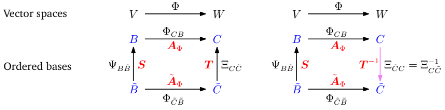
\includegraphics[width=\linewidth, height=2.5cm, keepaspectratio]{Pictures/maths/basis-change.png}
    \caption{Basis Change}
\end{figure}

\noindent\textbf{Notations}:
\begin{enumerate}
    \item linear mapping:  $\Phi : \mathbf{V \to W}$

    \item ordered bases of $\mathbf{V}$ : \(         \mathit{B} = \mathbf{(b_1, \cdots , b_n)} \quad\quad \tilde{\mathit{B}} = \mathbf{( \tilde{b}1, \cdots , \tilde{b}_n)}     \)

    \item ordered bases of $\mathbf{W}$ : \( \mathit{C} = \mathbf{(c_1, \cdots , c_n)} \quad\quad \tilde{\mathit{C}} = \mathbf{( \tilde{c}1, \cdots , \tilde{c}_n)} \)

    \item Transformation matrix of $\Phi: \mathbf{V} \to \mathbf{W}$ wrt bases $\mathit{B}$ and $\mathit{C}$ : $\mathbf{A}_\Phi \in \mathbb{R}^{m \times n}$

    \item Transformation matrix of $\Phi: \mathbf{V} \to \mathbf{W}$ wrt bases $\tilde{\mathit{B}}$ and $\tilde{\mathit{C}}$ : $\tilde{\mathbf{A}}_\Phi \in \mathbb{R}^{m \times n}$

    \item $A_\Phi$ is \textbf{transformation matrix} of $\Phi_{CB}$ wrt ordered bases $B$, $C$\\

    \item $\Psi_{B\tilde{B}} : V \to V$ maps coordinates with respect to the new basis $\tilde{B}$ onto the (unique) coordinates with respect to the “old” basis $B$ (in $V$)

    \item $\Xi_{\tilde{C}C} : W \to W$ maps coordinates with respect to $C$ onto coordinates with respect to $\tilde{C}$

    \item  \begin{align}
        \Phi_{\tilde{C}\tilde{B}}  
        &= \Xi_{\tilde{C}C} \circ \Phi_{CB} \circ \Psi_{B\tilde{B}} \\ 
        &= \Xi^{-1}_{C\tilde{C}} \circ \Phi_{CB} \circ \Psi_{B\tilde{B}} \\ 
    \end{align} 
    
\end{enumerate}

\vspace{0.2cm}
\noindent \textbf{Note}:
\begin{enumerate}
    \item Transformation matrices of a linear mapping $\Phi : \mathbf{V \to W}$ change if we change the bases in $\mathbf{V}$ and $\mathbf{W}$.

    \item 
\end{enumerate}

\begin{theorem}[Basis Change]\label{theorem: Basis Change}
    For a linear mapping $\Phi : \mathbf{V \to W}$, ordered bases\\ 
    \(
        \mathit{B} = \mathbf{(b_1, \cdots , b_n)} \quad\quad \tilde{\mathit{B}} = \mathbf{( \tilde{b}1, \cdots , \tilde{b}_n)}  \hfill \text{ of }\mathbf{V}
    \)\\
    and\\
    \(
        \mathit{C} = \mathbf{(c_1, \cdots , c_n)} \quad\quad \tilde{\mathit{C}} = \mathbf{( \tilde{c}1, \cdots , \tilde{c}_n)}  \hfill \text{ of }\mathbf{W}
    \)\\
    and a transformation matrix $\mathbf{A}_\Phi$ of $\Phi$ with respect to $\mathit{B}$ and $\mathit{C}$, the corresponding transformation matrix $\tilde{\mathbf{A}}_\Phi$ with respect to the bases $\tilde{\mathit{B}}$ and $\tilde{\mathit{C}}$ is given as\\
    \( \tilde{\mathbf{A}}_\Phi = \mathbf{T^{-\top} \mathbf{A}_\Phi S} \)
\end{theorem}

\vspace{0.2cm}
\noindent \textbf{where}:
\begin{enumerate}
    \item $\mathbf{S} \in \mathbb{R}^{n\times n}$ is the transformation matrix of $id_V$ that maps coordinates with respect to $\tilde{\mathit{B}}$ onto coordinates with respect to $\mathit{B}$

    \item $\mathbf{T} \in \mathbb{R}^{m\times m}$ is the transformation matrix of $id_W$ that maps coordinates with respect to $\tilde{\mathit{C}}$ onto coordinates with respect to $\mathit{C}$.
\end{enumerate}

\vspace{0.2cm}
\noindent \textbf{Proof}:
\begin{enumerate}
    \item we can write the vectors of the new basis $\hat{\mathit{B}}$ of $\mathbf{V}$ as a linear combination of the basis vectors of $\mathit{B}$, such that\\
    \(
        \displaystyle \hat{\mathbf{b}}_j = s_{1j}\mathbf{b}_1 + \cdots + s_{nj}\mathbf{b}_n = \sum_{i=1}^{n} s_{ij}\mathbf{b}_i \hfill (j = 1,\cdots,n)
    \)\\
    and,\\
    \(
        \displaystyle \hat{\mathbf{c}}_k = t_{1k}\mathbf{c}_1 + \cdots + t_{mk}\mathbf{c}_m = \sum_{l=1}^{n} t_{lk}\mathbf{c}_l \hfill (k = 1,\cdots,m)
    \)

    \item $\mathbf{S} = ((s_{ij})) \in \mathbb{R}^{n\times n}$ as the transformation matrix that maps coordinates with respect to $\tilde{\mathit{B}}$ onto coordinates with respect to $\mathit{B}$\\
    $j$th column of $\mathbf{S}$ is the \textbf{coordinate} representation of  $\tilde{\mathbf{b}}_j$ with respect to $\mathit{B}$\\
    $\mathbf{S}$ is a \textbf{regular matrix}.
    
    
    \item $\mathbf{T} = ((T_{lk})) \in \mathbb{R}^{m\times m}$ as the transformation matrix that maps coordinates with respect to $\tilde{\mathit{C}}$ onto coordinates with respect to $\mathit{C}$\\
    $k$th column of $\mathbf{T}$ is the \textbf{coordinate} representation of $\tilde{\mathbf{c}}_k$ with respect to $\mathbf{C}$\\
    $\mathbf{T}$ is a \textbf{regular matrix}.

    \item \( \displaystyle
        \Phi(\tilde{\mathbf{b}}_j) = \sum_{k=1}^{m} \tilde{a}_{kj}\textcolor{blue}{\tilde{\mathbf{c}}_k} = \sum_{k=1}^{m} \tilde{a}_{kj} \textcolor{blue}{\sum_{l=1}^{m} t_{lk} \mathbf{c}_l} = \sum_{l=1}^{m}\left( \textcolor{Magenta}{\sum_{k=1}^{m} t_{lk}\tilde{a}_{kj}} \right)\mathbf{c}_l
    \)  \\
    \( \displaystyle
     \Phi(\textcolor{blue}{\tilde{\mathbf{b}}_j}) = \Phi \left( \textcolor{blue}{\sum_{i=1}^{m} s_{ij}\mathbf{b}_i} \right) = \sum_{i=1}^{m} s_{ij} \textcolor{red}{\Phi(\mathbf{b}_i)} = \sum_{i=1}^{m} s_{ij} \textcolor{red}{\sum_{i=1}^{m} a_{li}\mathbf{c}_l} = \sum_{l=1}^{m}\left( \textcolor{Magenta}{\sum_{i=1}^{n} a_{li}s_{ij}} \right)\mathbf{c}_l
    \)

    \item \( \displaystyle
        \sum_{k=1}^{m} t_{lk}\tilde{a}_{kj} = \sum_{i=1}^{n} a_{li}s_{ij} 
    \)\\
    \(
        \Rightarrow \mathbf{T\tilde{A}}_\Phi = \mathbf{A}_\Phi \mathbf{S} \in \mathbb{R}^{m\times n}
    \)\\
    \(
        \Rightarrow \mathbf{\tilde{A}}_\Phi = \mathbf{T^{-\top}A}_\Phi \mathbf{S}
    \)\\
    Hence, Proved!
    
\end{enumerate}








\section{Coordinate vector/ Coordinates ( $\alpha$ ) \cite{mfml-1}}\label{Coordinate vector}\label{Coordinates}

Consider a vector space $\mathbf{V}$ and an ordered basis $\mathit{B} = \mathbf{(b_1, \cdots , b_n)}$ of $\mathbf{V}$. For any $\mathbf{x \in V}$ we obtain a unique representation (linear combination) \( \mathbf{x} = \alpha_1\mathbf{b}_1 + \cdots + \alpha_n\mathbf{b}_n \) of $\mathbf{x}$ with respect to $\mathit{B}$. Then $\alpha_1, \cdots , \alpha_n$ are the \textbf{coordinates} of $\mathbf{x}$ with respect to $\mathit{B}$, and the vector \( \displaystyle \bm{\alpha} = \begin{bmatrix} \alpha_1 & \hdots & \alpha_n \end{bmatrix}^\top \in \mathbb{R}^n \) is the \textbf{coordinate vector}/ coordinate representation of $\mathbf{x}$ with respect to the ordered basis $\mathit{B}$.


\noindent SEE:
\begin{enumerate}
    \item \fullref{ordered basis}
    \item \fullref{Linear Combination} 
\end{enumerate}

\vspace{0.2cm}
\noindent \textbf{Note}:
\begin{enumerate}
    \item For an $n$-dimensional vector space $\mathbf{V}$ and an ordered basis $\mathit{B}$ of $\mathbf{V}$, the mapping $\Phi : \mathbb{R}^n \to \mathbf{V}$, $\Phi(\mathbf{e}_i) = \mathbf{b}_i$, $i = 1, \cdots , n$, is linear (and because of \theoremref{theorem: isomorphic} an \textbf{isomorphism}), where $(\mathbf{e}_1, \cdots , \mathbf{e}_n)$ is the standard basis of $\mathbb{R}^n$.
\end{enumerate}




\section{Rank ( $rk(\mathbf{A})$ ) \cite{mfml-1}}\label{matrix: Rank}

The number of linearly independent columns of a matrix $\mathbf{A} \in \mathbb{R}^{m \times n}$ equals the number of linearly independent rows and is called the rank rank of $\mathbf{A}$ and is denoted by $rk(\mathbf{A})$.

\begin{enumerate}
    \item $rk(\mathbf{A}) = rk(\mathbf{A}^\top)$, i.e., the column rank equals the row rank.

    \item The columns of $\mathbf{A} \in \mathbb{R}^{m \times n}$ span a subspace $U \subseteq \mathbb{R}^m$ with $\dim(U) = rk(\mathbf{A})$. 

    \item The rows of $\mathbf{A} \in \mathbb{R}^{m\times n}$ span a subspace $W \subseteq \mathbb{R}^n$ with $\dim(W) = rk(\mathbf{A})$. A basis of $W$ can be found by applying Gaussian elimination to $A^\top$.

    \item For all $\mathbf{A} \in \mathbb{R}^{n\times n}$ it holds that $\mathbf{A}$ is regular (invertible) if and only if $rk(\mathbf{A}) = n$.

    \item For all $\mathbf{A} \in \mathbb{R}^{m\times n}$ and all $\mathbf{b} \in \mathbb{R}^m$ it holds that the linear equation system $\mathbf{Ax = b}$ can be solved if and only if $rk(\mathbf{A}) = rk(\mathbf{A}|\mathbf{b})$, where $\mathbf{A}|\mathbf{b}$ denotes the augmented system.

    \item For $\mathbf{A} \in \mathbb{R}^{m\times n}$ the subspace of solutions for $\mathbf{Ax = 0}$ possesses dimension $n - rk(\mathbf{A})$. This subspace is called the \textbf{kernel space}\indexlabel{kernel space} or the \textbf{null space}\indexlabel{null space}.

    \item A matrix $\mathbf{A} \in \mathbb{R}^{m\times n}$ has \textbf{full rank}\indexlabel{matrix: full rank} if its rank equals the largest possible rank for a matrix of the same dimensions. This means that the rank of a full-rank matrix is the lesser of the number of rows and columns, i.e., $rk(A) = \min(m, n)$. A matrix is said to be \textbf{rank deficient}\indexlabel{matrix: rank deficient} if it does not have full rank.

\end{enumerate}


\section{Linear Mappings/ vector space homomorphism/ linear transformation ( $\Phi(\mathbf{x})$ ) \cite{mfml-1}}\label{Linear Mappings/ vector space homomorphism/ linear transformation}

\begin{figure}[h]
    \centering
    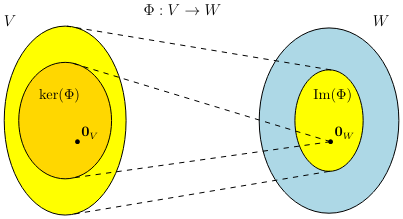
\includegraphics[width=\linewidth, height=2.5cm, keepaspectratio]{Pictures/maths/linear-mapping.png}
    \caption{Linear Mappings/ vector space homomorphism/ linear transformation}
\end{figure}

For vector spaces $V$, $W$, a mapping $\Phi : V \to W$ is called a linear mapping (or vector space homomorphism/ linear transformation) if:
\[
    \forall \mathbf{x, y} \in V, \forall\lambda, \psi \in \mathbb{R} : \Phi(\lambda\mathbf{x} + \psi\mathbf{y}) = \lambda\Phi(\mathbf{x}) + \psi\Phi(\mathbf{y})
\]

\begin{enumerate}
    \item we can represent linear mappings as matrices
    \item Consider a mapping $\Phi : \mathbb{V} \to \mathbb{W}$, where $\mathbb{V}$, $\mathbb{W}$ can be arbitrary sets. Then $\Phi$ is called
    \begin{enumerate}
        \item \textbf{Injective} if $\forall \mathbf{x, y} \in \mathbb{V}: \Phi(\mathbf{x}) = \Phi(\mathbf{y}) \Rightarrow \mathbf{x} = \mathbf{y}$ \indexlabel{Injective mapping}

        \item \textbf{Surjective} if $\Phi(\mathbb{V}) = \mathbb{W}$\indexlabel{Surjective mapping}\\
        If $\Phi$ is surjective, then every element in $\mathbb{W}$ can be “\textbf{reached}” from $\mathbb{V}$ using $\Phi$.

        \item \textbf{Bijective} if it is injective and surjective.\indexlabel{Bijective mapping}\\
        A bijective $\Phi$ can be “\textbf{undone}”, i.e., there exists a mapping $\Psi : \mathbb{W} \to \mathbb{V}$ so that $\Psi \circ \Phi(\textbf{x}) = \textbf{x}$. This mapping $\Psi$ is then called the \textbf{inverse} of $\Phi$ and normally denoted by $\Phi^{-1}$.\indexlabel{inverse linear mapping}
        
    \end{enumerate}

    \item \textbf{Isomorphism}\indexlabel{Isomorphism}: $\Phi : V \to W$ linear and bijective\\
    
    \begin{theorem}\label{theorem: isomorphic}
        Finite-dimensional vector spaces $V$ and $W$ are isomorphic if and only if $\dim(V) = \dim(W)$.
    \end{theorem}
    
    Intuitively, this means that vector spaces of the same dimension are kind of the same thing, as they can be transformed into each other without incurring any loss.\\
    This gives the justification to treat $\mathbb{R}^{m\times n}$ (the vector space of ${m\times n}$-matrices) and $\mathbb{R}^{mn}$ (the vector space of vectors of length $mn$) the same, as their dimensions are $mn$, and there exists a linear, bijective mapping that transforms one into the other.

    \item \textbf{Endomorphism}\indexlabel{Endomorphism}: $\Phi : V \to V$ linear

    \item \textbf{Automorphism}\indexlabel{Automorphism}: $\Phi : V \to V$ linear and bijective

    \item We define $id_V : V \to V , \mathbf{x} \to \mathbf{x}$ as the \textbf{identity mapping}\indexlabel{identity mapping} or \textbf{identity automorphism}\indexlabel{identity automorphism} in V.

    \item Consider vector spaces $V, W, X$. Then:
    \begin{enumerate}
        \item For linear mappings $\Phi : V \to W$ and $\Psi : W \to X$, the mapping $\Psi \circ \Phi : V \to X$ is also linear.

        \item If $\Phi : V \to W$ is an isomorphism, then $\Phi^{-1} : W \to V$ is an isomorphism, too.

        \item If $\Phi : V \to W$, $\Psi : V \to W$ are linear, then $\Phi + \Psi$ and $\lambda\Phi$, $\lambda \in \mathbb{R}$, are linear, too.
    \end{enumerate}
    
\end{enumerate}

\subsection{Matrix Representation of Linear Mappings \cite{mfml-1}}\label{Matrix Representation of Linear Mappings}

\begin{enumerate}
    \item Any $n$-dimensional vector space is \textbf{isomorphic} to $\mathbb{R}^n$. (SEE: \theoremref{theorem: isomorphic})
    
\end{enumerate}

\subsection{Transformation Matrix ( $\mathbf{A}_\Phi$ ) \cite{mfml-1}}\label{Transformation Matrix}

\begin{enumerate}
    \item Consider vector spaces $\mathbf{V}$, $\mathbf{W}$ with corresponding (ordered) bases $\mathit{B} = \mathbf{(b_1, \cdots , b_n)}$ and $\mathit{C} = \mathbf{(c_1, \cdots , c_m)}$. (SEE: \fullref{ordered basis})

    \item Moreover, we consider a linear mapping $\Phi : \mathbf{V} \to \mathbf{W}$. 

    \item For $j \in \{1, \cdots , n\}$, \(     \displaystyle \Phi(\mathbf{b}_j) = \alpha_{1j}\mathbf{c}_1 + \cdots + \alpha_{mj}\mathbf{c}_m = \sum_{i=1}^{m} \alpha_{ij}\mathbf{c}_{i} \) is the \textbf{unique} representation of $\Phi(\mathbf{b}_j)$ with respect to $\mathit{C}$. 

    \item The $m \times n$-matrix $\mathbf{A}_\Phi$, whose elements are given by \( \mathbf{A}_\Phi(i, j) = \alpha_{ij} \), is called \textbf{transformation matrix} of $\Phi$ (with respect to the ordered bases $\mathit{B}$ of $\mathbf{V}$ and $\mathit{C}$ of $\mathbf{W}$)

    \item The coordinates of $\Phi(\mathbf{b}_j)$ with respect to the ordered basis $\mathit{C}$ of $\mathbf{W}$ are the $j$-th column of $\mathbf{A}_\Phi$. (SEE: \fullref{Coordinate vector})

    \item Consider (\textbf{finite-dimensional}) vector spaces $\mathbf{V, W}$ with ordered bases $\mathit{B, C}$ and a linear mapping $\Phi : \mathbf{V \to W}$ with transformation matrix $\mathbf{A}_\Phi$. \\
    If $\hat{\mathbf{x}}$ is the coordinate vector of $\mathbf{x} \in \mathbf{V}$ with respect to $\mathit{B}$ and $\hat{\mathbf{y}}$ the coordinate vector of $\mathbf{y} = \Phi(\mathbf{x}) \in \mathbf{W}$ with respect to $\mathit{C}$, then $\hat{\mathbf{y}} = \mathbf{A}_\Phi\hat{\mathbf{x}}$.

    \item The transformation matrix can be used to map coordinates with respect to an ordered basis in $\mathbf{V}$ to coordinates with respect to an ordered basis in $\mathbf{W}$.

    \item for linear mappings $\Phi : V \to W$ and $\Psi : W \to X$ the mapping $\Psi \circ \Phi : V \to X$ is also \textbf{linear}.\\
    With transformation matrices $\mathbf{A}_\Phi$ and $\mathbf{A}_\Psi$ of the corresponding mappings, the overall transformation matrix is $\mathbf{A}\Psi\circ\Phi = \mathbf{A}_\Psi \mathbf{A}_\Phi$

    \begin{enumerate}
        \item[] \fullref{Basis Change}

        \item $\mathbf{A}_\Phi$ is the transformation matrix of a linear mapping $\Phi_{CB} : V \to W$ with respect to the bases $B$, $C$.

        \item $\tilde{\mathbf{A}}_\Phi$ is the transformation matrix of the linear mapping $\tilde{\mathbf{A}}_\Phi : V \to W$ with respect to the bases $\tilde{B}, \tilde{C}$ 

        \item $\mathbf{S}$ is the \textbf{transformation matrix} of a linear mapping $\Psi_{B\tilde{B}} : V \to V$ (\textbf{automorphism}) that represents  in terms of $B$. Normally, $\Psi = id_V$ is the identity mapping in $V$

        \item $\mathbf{T}$ is the \textbf{transformation matrix} of a linear mapping $\Xi_{C\tilde{C}} : W \to W$ (\textbf{automorphism}) that represents  in terms of $C$. Normally, $\Xi = id_W$ is the identity mapping in $W$

        \item Informally, transformations just in terms of bases, then:
        \[
            \hfill
            \mathbf{A}_\Phi : B \to C
            \hfill
            \tilde{\mathbf{A}}_\Phi : \tilde{B} \to \tilde{C}
            \hfill
            \mathbf{S} : \tilde{B} \to B
            \hfill
            \mathbf{T} : \tilde{C}  \to C
            \hfill
            \mathbf{T}^{-1}: C \to \tilde{C}
            \hfill
        \]
        \[
            \hfill
            \tilde{B} \to \tilde{C}
            =
            \tilde{B} \to B \to C \to \tilde{C}
            \hfill 
            \tilde{\mathbf{A}}_\Phi = \mathbf{T}^{-1}\mathbf{A}_\Phi \mathbf{S}
            \hfill
        \]
        \[
            \hfill
            \mathbf{x} 
            \mapsto \mathbf{Sx}
            \mapsto \mathbf{A}_\Phi(\mathbf{Sx})
            \mapsto \mathbf{T}^{-1}(\mathbf{A}_\Phi(\mathbf{Sx}))
            = \mathbf{\tilde{A}}_\Phi \mathbf{x}
            \hfill
        \]

        \textbf{Note}: execution order is from right to left because vectors are multiplied at the right-hand side 
        
    \end{enumerate}
    
\end{enumerate}



%%%%%%%%%%%%%%%%%%%%%%%%%%%%%%%%%%%%%%%%%%%%%%%%%%%%%%%%%%



\section{Kernel/ null space ( $ker(\Phi)$ ) \cite{mfml-1}}\label{Kernel/ null space}

For $\Phi : V \to W$, we define the kernel/ null space 
\[
    \hfill
    ker(\Phi) := \Phi^{-1}(0_W) = \{v \in V : \Phi(v) = 0_W\}
    \hfill
\]

\begin{enumerate}
    \item kernel is the set of vectors $v \in V$ that $\Phi$ maps onto the neutral element $0_W \in W$

    \item It \textbf{ALWAYS} holds that $\Phi(0_V) = 0_W$ and, therefore, $0_V \in ker(\Phi)$

    \item the null space is \textbf{NEVER} empty

    \item $ker(\Phi) \subseteq V$ is a subspace of $V$

    
\end{enumerate}


%%%%%%%%%%%%%%%%%%%%%%%%%%%%%%%%%%%%%%%%%%%%%%%%%%%%%%%%%%


\section{Image/ range ( $Im(\Phi)$ ) \cite{mfml-1}}\label{Image/ range}

For $\Phi : V \to W$, we define the image/ range 
\[
    \hfill
    Im(\Phi) := \Phi(V) = \{w \in W | \exists v \in V : \Phi(v) = w\}
    \hfill
\]

\begin{enumerate}
    \item image is the set of vectors $w \in W$ that can be “reached” by $\Phi$ from any vector in $V$

    \item $Im(\Phi) \subseteq W$ is a subspace of $W$
\end{enumerate}



%%%%%%%%%%%%%%%%%%%%%%%%%%%%%%%%%%%%%%%%%%%%%%%%%%%%%%%%%%

\section{Domain and Codomain \cite{mfml-1}}\label{Domain and Codomain}

if $\Phi : V \to W$, then:
\begin{enumerate}
    \item $V$ is domain
    \item $W$ is codomain
\end{enumerate}

%%%%%%%%%%%%%%%%%%%%%%%%%%%%%%%%%%%%%%%%%%%%%%%%%%%%%%%%%%

\section{Null Space and Column Space \cite{mfml-1}}\label{Null Space and Column Space}

Let us consider $\mathbf{A} \in \mathbb{R}^{m\times n}$ and a linear mapping $\Phi : \mathbb{R}^n \to \mathbb{R}^m$, $\mathbf{x} \mapsto \mathbf{Ax}$.

\begin{enumerate}
    \item For $\mathbf{A} = [\mathbf{a}_1, \cdots , \mathbf{a}_n]$, where $\mathbf{a}_i$ are the columns of $\mathbf{A}$:
    \begin{align*}
        \displaystyle
        Im(\Phi) 
        &= \{ \mathbf{Ax} : \mathbf{x} \in \mathbb{R}^n \} \\
        &= \left\{ \sum_{i=1}^{n} x_i\mathbf{a}_i : \forall x_i \in \mathbb{R}, i=1,\cdots,n \right\} \\
        &= span[\mathbf{a}_1,\cdots, \mathbf{a}_n] \subseteq \mathbb{R}^m \\
    \end{align*}

    the image is the span of the columns of A, also called the \textbf{column space}\indexlabel{column space}. Therefore, the column space (image) is a subspace of $\mathbb{R}^m$, where m is the \textbf{“height” of the matrix}\indexlabel{height of the matrix}.

    \item $rk(\mathbf{A}) = dim(Im(\Phi))$

    \item The kernel/null space $ker(\Phi)$ is the general solution to the homogeneous system of linear equations $\mathbf{Ax = 0}$ and captures all possible linear combinations of the elements in $\mathbb{R}^n$ that produce $\mathbf{0} \in \mathbb{R}^m$.

    \item The kernel is a subspace of $\mathbb{R}^n$, where $n$ is the \textbf{“width” of the matrix}\indexlabel{width of the matrix}.

    \item The kernel focuses on the relationship among the columns, and we can use it to determine whether/ how we can express a column as a linear combination of other columns.
\end{enumerate}



%%%%%%%%%%%%%%%%%%%%%%%%%%%%%%%%%%%%%%%%%%%%%%%%%%%%%%%%%%


\section{Rank-Nullity Theorem ( $dim(ker(\Phi)) + dim(Im(\Phi)) = dim(V)$ ) \cite{mfml-1}}\label{Rank-Nullity Theorem}

For vector spaces $V, W$ and a linear mapping $\Phi : V \to W$ it holds that 

\[
    \hfill
    dim(ker(\Phi)) + dim(Im(\Phi)) = dim(V)
    \hfill
\]

The rank-nullity theorem is also referred to as the \textbf{fundamental theorem of linear mappings}\indexlabel{fundamental theorem of linear mappings}.

\begin{enumerate}
    \item If $dim(Im(\Phi)) < dim(V)$, then $ker(\Phi)$ is non-trivial, i.e., the kernel contains more than $0_V$ and $dim(ker(\Phi)) \geq 1$

    \item If $\mathbf{A}_\Phi$ is the transformation matrix of $\Phi$ with respect to an ordered basis and $dim(Im(\Phi)) < dim(V)$, then the system of linear equations $\mathbf{A}_\Phi x = 0$ has infinitely many solutions

    \item If $dim(V) = dim(W)$, then the following three-way equivalence holds: 
    \begin{enumerate}
        \item $\Phi$ is injective

        \item $\Phi$ is surjective

        \item $\Phi$ is bijective 
    \end{enumerate}
    since $Im(\Phi) \subseteq W$

    
\end{enumerate}



%%%%%%%%%%%%%%%%%%%%%%%%%%%%%%%%%%%%%%%%%%%%%%%%%%%%%%%%%%



\section{Affine Subspace/ linear manifold ( $L = x0 + U$ ) \cite{mfml-1}}\label{Affine Subspace/ linear manifold}

Let $V$ be a vector space, $x_0 \in V$ and $U \subseteq V$ a subspace. Then the subset

\begin{table}[h]
    \begin{minipage}{0.49\linewidth}
        \begin{align*}
            L &= x_0 + U\\
             &= \{x_0 + u : u \in U\} \\
             &= \{v \in V | \exists u \in U : v = x_0 + u\} \subseteq V
        \end{align*}
    \end{minipage}
    \hfill
    \begin{minipage}{0.49\linewidth}
        \begin{table}[H]
            \begin{tabular}{l l}
                $U$ & direction or direction space \\
                $x_0$ & support point \\
            \end{tabular}
        \end{table}
    \end{minipage}
\end{table}

is called affine subspace or linear manifold of $V$. 


\begin{enumerate}
    \item an affine subspace is not a (linear) subspace (vector subspace) of $V$ for $x_0 \not\in U$

    \item Consider two affine subspaces $L = x_0 + U$ and  of a vector space $V$\\
    $L \subseteq \tilde{L}$ if and only if $U \subseteq \tilde{U}$ and $x_0 - \tilde{x}_0 \in \tilde{U}$
    
    \item Describing affine space using parameters:
    \begin{enumerate}
        \item Consider a k-dimensional affine space $L = x_0 + U$ of $V$

        \item If $\mathbf{(b_1, \cdots , b_k)}$ is an ordered basis of $U$, then every element $x \in L$ can be uniquely described as
        \[
            \hfill 
            x = x_0 + \lambda_1b_1 + \cdots + \lambda_kb_k 
            \hfill
        \]
        where $\lambda_1, \cdots , \lambda_k \in \mathbb{R}$

        \item This representation is called \textbf{parametric equation}\indexlabel{parametric equation} of $L$ with directional vectors $b_1, \cdots , b_k$ and parameters $\lambda_1, \cdots , \lambda_k$
        
    \end{enumerate}
    
\end{enumerate}


%%%%%%%%%%%%%%%%%%%%%%%%%%%%%%%%%%%%%%%%%%%%%%%%%%%%%%%%%%


\section{System of Linear Equations \cite{mfml-1}}\label{System of Linear Equations}

\subsection*{Setup/ Scenario}

\textbf{Equations}:

\noindent\textbf{Common/ Classical representation}:
\[
    \begin{matrix}
        a_{11}x_1 + a_{12}x_2 + \cdots + a_{1n}x_n = b_1\\
        \vdots \\
        a_{m1}x_1 + a_{m2}x_2 + \cdots + a_{mn}x_n = b_m
    \end{matrix}
\]       
\textbf{Matrix-vector representations/ Compact representations} ( $Ax=b$ ):
\[
    \begin{bmatrix}
        a_{11}\\ \vdots\\ a_{m1}
    \end{bmatrix} x_1 +
    \begin{bmatrix}
        a_{12}\\ \vdots\\ a_{m2}
    \end{bmatrix} x_2 +
    \cdots
    \begin{bmatrix}
        a_{1n}\\ \vdots\\ a_{mn}
    \end{bmatrix} x_n
    =
    \underset{A}{
        \underbrace{
            \begin{bmatrix}
                a_{11} & \cdots & a_{1n}\\
                \vdots & \ddots & \vdots \\
                a_{m1} & \cdots & a_{mn}\\
            \end{bmatrix}
        }
    }
    \underset{x}{
        \underbrace{
            \begin{bmatrix}
                x_1 \\ \vdots \\ x_n
            \end{bmatrix}
        }
    }
    =
    \underset{b}{
        \underbrace{
            \begin{bmatrix}
                b_{1}\\ \vdots\\ b_{m}
            \end{bmatrix}
        }
    }
\]


\begin{table}[h]
    \begin{tabular}{l l l}
        no of \textbf{equations} & $m$ & $(i=1,\cdots,m)$\\
        no of \textbf{variables} & $n$ & $(j=1,\cdots,n)$ \\
        \textbf{unknowns} & $x = (x_1,\cdots,x_n) \in R^n$\\
        \textbf{knowns} & $a_{ij}, b_{i} \in R$
    \end{tabular}
\end{table}


\subsection{Homogeneous systems of linear equations ( $\mathbf{Ax = 0}$ ) \cite{mfml-1, chatgpt}}\label{Homogeneous systems of linear equations}

\begin{enumerate}
    \item For homogeneous equation systems $\mathbf{Ax = 0}$ the solution was a vector subspace, which we can also think of as a special affine space with support point $\mathbf{x}_0 = \mathbf{0}$.

    \item A homogeneous system of linear equations is one in which \textbf{ALL} the constant terms are zero.
\end{enumerate}

\vspace{0.2cm}
\textbf{Properties}:
\begin{enumerate}
    \item \textbf{Trivial Solution}: The system always has at least one solution, the trivial solution $\mathbf{x}=0$.

    \item \textbf{Non-Trivial Solutions}: If the number of equations is less than the number of unknowns ($m<n$), there are typically an infinite number of solutions. This occurs because the system is underdetermined.

    \item \textbf{Solution Space}: The solutions form a subspace of $\mathbb{R}^n$, specifically the null space of the matrix $\mathbf{A}$.
\end{enumerate}



\subsection{Inhomogeneous systems of linear equations ( $\mathbf{Ax = b}$ ) \cite{mfml-1, chatgpt}}\label{Inhomogeneous systems of linear equations}


\begin{enumerate}
    \item For $\mathbf{A} \in \mathbb{R}^{m\times n}$ and $\mathbf{x} \in \mathbb{R}^m$, the solution of the system of linear equations $\mathbf{A\boldsymbol{\lambda} = x}$ is either the empty set or an affine subspace of Rn of dimension $n - rk(\mathbf{A})$.

    \item The solution of the linear equation $\lambda_1\mathbf{b}_1 + \cdots + \lambda_n\mathbf{b}_n = \mathbf{x}$, where $(\lambda_1, \cdots , \lambda_n) \neq (0, \cdots , 0)$, is a hyperplane in $\mathbb{R}^n$.

    \item In $\mathbb{R}^n$, every $k$-dimensional affine subspace is the solution of an inhomogeneous system of linear equations $\mathbf{Ax = b}$, where $\mathbf{A} \in \mathbb{R}^{m\times n}$, $\mathbf{b} \in \mathbb{R}^m$ and $rk(\mathbf{A}) = n - k$.

    \item An inhomogeneous system of linear equations includes non-zero constant terms.
\end{enumerate}

\vspace{0.2cm}
\textbf{Properties}:
\begin{enumerate}
    \item \textbf{Existence of Solutions}: Solutions exist if and only if the vector $\mathbf{b}$ lies in the column space of $\mathbf{A}$. This is determined by checking if the system $\mathbf{[A|b]}$ is consistent (i.e., there are no contradictions in the augmented matrix).

    \item \textbf{Uniqueness of Solutions}: If the matrix $\mathbf{A}$ has full column rank and $m=n$ (i.e., the matrix is square and invertible), the system has a unique solution. If A does not have full column rank, the system may have no solutions or infinitely many solutions.

    \item \textbf{Particular and General Solutions}: If a particular solution $\mathbf{x}_p$ exists, the general solution can be written as $\mathbf{x}=\mathbf{x}_p +\mathbf{x}_h$, where $\mathbf{x}_h$ is the general solution to the corresponding homogeneous system $\mathbf{Ax=0}$.
\end{enumerate}

\subsection{Consistent System}\label{Consistent System of equations}

\begin{enumerate}
    \item A system of equations is considered consistent if there exists \textbf{AT LEAST ONE SOLUTION} that satisfies all the equations.
\end{enumerate}


\subsection{Dependent Solution}\label{Dependent Solution of linear equations}

\begin{enumerate}
    \item happens when no of equations $<$ no of variables
    
    \item Solutions are dependent if one can be expressed as a linear combination of the others.
\end{enumerate}

\subsection{Types of Solutions}
\begin{enumerate}
    \item \textbf{No solution}
    \begin{enumerate}
        \item Inconsistent
    \end{enumerate}
    
    \item \textbf{Unique solution}
    \begin{enumerate}
        \item Consistent
        \item Independent
    \end{enumerate}

    \item \textbf{Infinitely many solutions}
    \begin{enumerate}
        \item Consistent
        \item Dependent
    \end{enumerate}

    \item \textbf{Trivial solution}
    \begin{enumerate}
        \item $x_i = 0, \forall x_i$, is a solution
        \item Consistent
        \item Dependent
    \end{enumerate}

\end{enumerate}


\subsection{Elementary Transformations \cite{mfml-1}} \label{Elementary Transformations}
transformations that keep the solution set the same, but that transform the equation system into a simpler form:
\begin{enumerate}
    \item Exchange of two equations (rows in the matrix representing the system of equations)
    \[ R_i \Leftrightarrow R_j \]

    \item Multiplication of an equation (row) with a constant $\lambda \in R\backslash \{0\}$
    \[ R_i := \lambda R_i \]

    \item Addition of two equations (rows)
    \[ R_i := R_i + R_j \]

\end{enumerate}


\subsection{Solutions of system of linear equations \cite{mfml-1}}\label{Solutions of system of linear equations}

\begin{table}[h]
    \begin{tabular}{l l}
        Original System	& $Ax = b$ \\

        Homogeneous System & $Ax = 0$ \\
    \end{tabular}
\end{table}

\begin{align*}
   & Ax = b \\
   & \Rightarrow A(x_0 + \lambda _1x_1 + \lambda _2x_2 + \cdots ) = b	&&& (\lambda _i \in R) \\
   & \Rightarrow Ax_0 + \lambda _1Ax_1 + \lambda _2Ax_2 + \cdots  = b + 0 + 0 + \cdots  = b
\end{align*}

\begin{table}[h]
    \begin{tabular}{l l l}
        $x = x0$ & particular solution & ($Ax = b$ part) \\
        
        $x = x_1, x_2, \cdots$ & solutions to homogeneous equation & ($Ax = 0$ part)
    \end{tabular}
\end{table}

\subsubsection{Augmented Matrix ( $[A|b]$ ) \cite{mfml-1}} \label{Augmented Matrix}

An augmented matrix for a system of equations is a matrix of numbers in which each row represents the constants from one equation (both the coefficients and the constant on the other side of the equal sign) and each column represents all the coefficients for a single variable.


\subsubsection{Row-Echelon Form (REF) \cite{mfml-1,wiki/Row_echelon_form}}\label{Row-Echelon Form (REF)}

\begin{enumerate}
    \item A matrix is in row echelon form if it can be obtained as the result of \textbf{Gaussian elimination}.

    \item Every matrix can be put in row echelon form by applying a sequence of \textbf{elementary row operations}.

    \item can be viewed as a generalization of \textbf{upper triangular} form for rectangular matrices

    \item pivots may not be $1$
\end{enumerate}


\subsubsection{Reduced Row Echelon Form (RREF) \cite{mfml-1,wiki/Row_echelon_form}}\label{Reduced Row Echelon Form (RREF)}
A matrix is in row-echelon form if:
\begin{enumerate}
    \item All rows that contain only zeros are at the bottom of the matrix; correspondingly, all rows that contain at least one nonzero element are on top of rows that contain only zeros.

    \item Looking at nonzero rows only, the first nonzero number from the left (also called the pivot or the leading coefficient) is always strictly to the right of the pivot of the row above it.
\end{enumerate}

\noindent\textbf{Note}:
\begin{enumerate}
    \item A matrix is in row echelon form if it can be obtained as the result of \textbf{Gauss–Jordan elimination}

    \item it is in row echelon form, with the additional property that the first nonzero entry of each row is equal to $1$ and is the only nonzero entry of its column

    \item The reduced row echelon form of a matrix is \textbf{unique} and does not depend on the sequence of elementary row operations used to obtain it

    \item pivots \textbf{MUST} be $1$
\end{enumerate}

\subsubsection{Particular Solution (or special solution) \cite{mfml-1}} \label{Particular Solution (or special solution)}
solution of $Ax = b$

\paragraph{Direct Solution  \cite{mfml-1}}

\textbf{Conditions}:
\begin{enumerate}
    \item A is a \textbf{square matrix} and \textbf{invertible}
\end{enumerate}

\[ Ax = b \Leftrightarrow x = A^{-1}b \]

\textbf{Disadvantage}:
\begin{enumerate}
    \item not good at numerical precision
\end{enumerate}


\paragraph{Pseudo Direct Solution \cite{mfml-1}}
\textbf{Conditions}:
\begin{enumerate}
    \item $A$ needs to have \textbf{linearly independent columns}
\end{enumerate}

\[
    Ax = b 
    \Leftrightarrow 
    A^\top Ax = A^\top b 
    \Leftrightarrow
    x = (A^\top A)^{-1}A^\top b
\]

\textbf{Disadvantage:}
\begin{enumerate}
    \item requires many computations for the matrix-matrix product and computing the inverse of $A^\top A$

    \item not good at numerical precision
\end{enumerate}



\paragraph{Using Gaussian Elimination}
\textbf{Steps:}
\begin{enumerate}
    \item use RREF on Augmented matrix $[A|b]$

    \item express the right-hand side of the equation system using the pivot columns, such that ${\displaystyle b = \sum_{i=1}^{P} \lambda_i p_i}$ where $p_i$ are pivot columns.

    \item $\lambda _i$ are determined easiest if we start with the rightmost pivot column and work our way to the left

    \item solution = $x_0 = [\lambda _1, \lambda _2, \cdots, \lambda _P]^\top$
\end{enumerate}

\subsubsection{Solutions of $Ax=0$ \cite{mfml-1}}

Every subspace $U \subseteq (R^n , +, \cdot)$ is the solution space of a homogeneous system of linear equations $Ax = 0$ for $x \in R^n$
\begin{enumerate}
    \item As it is a homogeneous system, there can’t be “No Solution”

    \item Solutions will be:
    \begin{enumerate}
        \item Unique solution (trivial) = $0^n \in R^n$
        \item infinite solutions
    \end{enumerate}
\end{enumerate}


\paragraph{The Minus-$1$ Trick \cite{mfml-1}}\label{Solutions of ax=0: The Minus-1 Trick}
\textbf{Steps}:
\begin{enumerate}
    \item $A := RREF(A)$

    \item ignore the rows with only 0s
    \[
        A = 
        \begin{bmatrix}
            0 & \cdots  & 0 & 1 & \ast & \cdots  & \ast & 0 & \ast & \cdots  & \ast & 0 & \ast & \cdots  & \ast\\
            \vdots && \vdots & 0 & 0 & \cdots  & 0 & 1 & \ast & \cdots  & \ast & \vdots & \vdots & & \vdots\\
            \vdots & & \vdots & \vdots & \vdots & & \vdots & 0 & \vdots & & \vdots & \vdots & \vdots && \vdots\\
            \vdots & & \vdots & \vdots & \vdots & & \vdots & \vdots & \vdots & & \vdots & 0 & \vdots && \vdots\\
            0 & \cdots & 0 & 0 & 0 & \cdots & 0 & 0 & 0 & \cdots & 0 & 1 & \ast & \cdots & \ast\\
        \end{bmatrix}
    \]
    where $\ast$ can be an arbitrary real number, with the constraints that the \textbf{first nonzero entry} per row must be $1$ and all other entries in the corresponding column must be $0$. 

    \item columns $j_1, \cdots , j_k$ with the pivots are the standard unit vectors $e_1, \cdots , e_k \in R^k$

    \item extend this matrix to an $n \times n$-matrix $B$ by adding $n - k$ rows of the form
    \[
        \begin{bmatrix}
            0 & \cdots & 0 & -1 & 0 & \cdots & 0
        \end{bmatrix}
    \]
    so that the \textbf{diagonal} of the augmented matrix $B$ contains either $1$ or $-1$

    \item columns of $B$ that contain the $-1$ as pivots are solutions of the homogeneous equation system $Ax = 0$

\end{enumerate}

\paragraph{Classical method \cite{mfml-1}}\label{Solutions of ax=0: Classical method}

\textbf{Steps}:
\begin{enumerate}
    \item $A := RREF(A)$

    \item express the pivot variables in terms of free variables

    \item for each free variable, put it $1$ and rest free variables as $0$s

    \item get $n-k$ solutions

\end{enumerate}


\subsubsection{General Solution to $Ax=b$ \cite{mfml-1}}\label{General Solution to Ax=b}

General Solution = Particular Solution (solution of $Ax=b$) + $\lambda_i$ * (solutions of $Ax = 0$)


\subsection{Systems of linear equations and affine subspaces \cite{mfml-1}}\label{Systems of linear equations and affine subspaces}
\begin{enumerate}
    \item For $A \in  R^{m\times n}$ and $x \in  R^m$, the solution of the system of linear equations $A\lambda  = x$ is either the empty set or an affine subspace of $Rn$ of dimension $n - rk(A)$. 

    \begin{enumerate}
        \item In particular, the solution of the linear equation $\lambda _1b_1 + \cdots  + \lambda _nb_n = x$, where $(\lambda _1, \cdots  , \lambda _n) \neq (0, \cdots  , 0)$, is a hyperplane in $R^n$
    \end{enumerate}

    \item In $R^n$, \textbf{EVERY} $k$-dimensional affine subspace is the solution of an inhomogeneous system of linear equations $Ax = b$, where $A \in  R^{m\times n}$, $b \in  R^m$ and $rk(A) = n - k$

    \item for homogeneous equation systems $Ax = 0$ the solution was a vector subspace, which we can also think of as a special affine space with support point $x0 = 0$
\end{enumerate}




%%%%%%%%%%%%%%%%%%%%%%%%%%%%%%%%%%%%%%%%%%%%%%%%%%%%%%%%%%%


\section{Affine Mapping \cite{mfml-1}}\label{Affine Mapping}

For two vector spaces $V, W$, a linear mapping $\Phi : V \to W$, and $\mathbf{a} \in W$, the mapping

\[
    \hfill
    \phi : V \to W
    \hfill
    \mathbf{x} \mapsto \mathbf{a} + \Phi(\mathbf{x})
    \hfill
\]

is an affine mapping from $V$ to $W$. The vector $\mathbf{a}$ is called the \textbf{translation vector}\indexlabel{affine mapping: translation vector} of $\phi$.

\begin{enumerate}
    \item Every affine mapping $\phi : V \to W$ is also the composition of a linear mapping $\Phi : V \to W$ and a translation $\tau : W \to W$ in $W$, such that $\phi = \tau \circ \Phi$. The mappings $\Phi$ and $\tau$ are uniquely determined.

    \item The composition $\phi' \circ \phi$ of affine mappings $\phi : V \to W$, $\phi': W \to X$ is affine.

    \item Affine mappings keep the geometric structure invariant. 
    
    \item They also preserve the dimension and parallelism.
\end{enumerate}














\vspace{4cm}
\url{https://drive.google.com/file/d/1JS4tlbMRYv8oHYrLgISR_NV9y6-_2j5h/edit}\\
76 / 417











































































































































































